\part{Capítulo uno}
%\graphicspath{ {img/} }

%----------------------------------------------------------------------------------------
%	CHAPTER 1
%----------------------------------------------------------------------------------------

\chapterimage{ima2} % Chapter heading image



\chapter{Interés simple}


\section{Fórmulas de capítulo }

\begin{spacing}{1.5}
\begin{center}
\begin{tabular}{ |p{6cm}|p{5cm}| p{4cm}|}
\hline 
\rowcolor{orange!50}
\begin{center}\textbf{Fórmula} \end{center} & \begin{center} \textbf{Nombre}\end{center} & \begin{center} \textbf{Excel} \end{center} \\ \hline                        

I = Pin & Valor interés simple & TASA.INT(ni;nf;P)\\ \hline

F = P+I & Valor futuro &  - \\ \hline 

P= $\frac{F}{1+ni }$ & Valor presente & - \\ \hline

F= P(1+in) & Valor futuro  & - \\ \hline

P= F(1-dn) & Valor presente de un flujo futuro & - \\ \hline

F= P/(1-dn) & Valor futuro de un flujo presente & - \\ \hline

VL= F(1-dn) & Valor líquido dado un flujo futuro & - \\ \hline

 
\end{tabular}
\end{center}
\end{spacing}

\section{Introducción}
En este capítulo daremos definiciones y conceptos básicos utilizados en las finanzas, los cuales serán indispensables para el desarrollo de la guía. Este enfoque analítico nos permite la optimización de los recursos económicos, lo cual viene a ser el objetivo final de esta guía.

\section{Valor del dinero a través del tiempo}
No es lo mismo tener hoy \$100.000 que tener \$100.000 dentro de un año, porque lo que hoy se puede hacer con ese dinero es más de lo que se podrá hacer dentro de un año debido a que normalmente todos los artículos suben de precio, por tal motivo cuando se habla de una suma de dinero debe especificarse la fecha o de lo contrario la información es incompleta. Lo anterior se puede expresar en una forma muy simple: El dinero cambia de valor a través del tiempo.
\\\\
El concepto anterior está íntimamente ligado con el concepto de equivalencia que consiste en que, sumas de dinero diferentes en épocas distintas tienen el mismo poder adquisitivo, así por ejemplo si dentro de un año necesito \$120.000 para hacer lo que hoy hago con \$100.000 entonces diré que estas sumas son equivalentes en el tiempo.

\section{Interés (I)}

Todos los bienes son susceptibles de ser entregados a otra persona en arriendo y por ello cobrar un canon de arrendamiento, por lo que es posible dar una casa en arriendo y cobrar una suma mensual por el uso de esa casa, también es posible entregar en arriendo un vehículo o una máquina etc. De la misma forma es posible entregar en arriendo un dinero y el canon del arrendamiento del dinero recibe el nombre de interés el cual representaremos por I.
\\\\
Otra forma de ver el concepto de interés es como la retribución económica que devuelve el capital inicial por período transcurrido, de forma tal que compense la desvalorización de la moneda, que cubra el riesgo y que pague el alquiler del dinero como premio al dueño por no haberlo consumido.

\section{Tasa de interés periódico (i)}
Es el porcentaje (\%) que se paga por el alquiler del dinero, lo representaremos por i . Por ejemplo si tengo que pagar \$4 de interés por un préstamo de \$100 en un año, entonces la tasa de interés será del 4 \% período anual vencido que se puede escribir como 4\% pav y si tengo que pagar 3 centavos por el préstamo de \$1 la tasa será  3\% pav o equivalente a 0,03 pav.

\section{Tiempo (t)}
Es la duración de la inversión; y lo representaremos por $t$ y no por $n$ que corresponde al período de ingreso o pago de interés. % el período de liquidación de los intereses. En interés simple la unidad de tiempo es el año.

\section{Período (n)}
Tiempo unitario de liquidación de intereses, puede ser diario, semanal, mensual, bimensual, trimestral, semestral, anual, bianual, entre otros. %El periodo es equivalente = Días de liquidación de Intereses/ Días del año 

\section{Capital inicial (P)}
Es la cantidad de dinero que se invierte, también se le conoce con el nombre de principal, valor actual, valor inicial o valor presente y lo representaremos por P.

\section{Postulado básico de las finanzas}
El postulado básico de las finanzas establece que el interés es una función directa que depende de 3 variables: el capital inicial (\textit{mientras más grande sea el capital mayor deberá ser el interés) la tasa (la tasa depende de las fuerzas del mercado, cuando hay escasez de dinero o cuando los precios en general están al alza la tasa será mayor) y del tiempo (mientras más tiempo dure la inversión mayor será el interés}). Ver la tasa EA de la SuperFinanciera.

\section{Fórmula de interés (I)}
De acuerdo con el postulado anterior podemos establecer la siguiente ecuación:
\begin{equation}
I = Pin \hspace{35pt} \textit{Valor interés simple (I)}
\end{equation}

\section{Gráfica de flujo de caja}
\textit{A fin de facilitar la comprensión de los problemas mediante una gráfica, se ha adoptado la siguiente convención: la línea horizontal representa el tiempo y allí escribiremos las fechas y los períodos de tiempo; de esta línea salen unas flechas hacia arriba y otras hacia abajo, las que están hacia arriba representan ingresos y las que están hacia abajo representan egresos}.
\\\\
\textit{Nota.} En este texto las fechas las daremos en la forma:  AAAA-MM-DD (Año-mes-día) por ejemplo, el día 15 de septiembre de 1998 1o representaremos así:         15-09-98

\section{Capital final (F, i, n, P)}
Es el capital inicial más los intereses, también se le denomina monto, valor final, valor futuro, la suma o acumulado y lo representaremos por $F$. De acuerdo a la definición la fórmula será:

\begin{align*}
    F=P+I \hspace{35pt} \textit{Valor futuro de un flujo (P)}\\
    F= P(1+in)\hspace{35pt} \textit{Valor futuro de un flujo (p)}\\
\end{align*}

\textbf{Ejemplo 1}\\
Calcular el valor futuro de \$30.000 desde el 23 de agosto de 1999 hasta el 27 de octubre del mismo año al 35\% periodo vencido. Utilice año de 365 días. \\

\textbf{Solución}\\
El problema consiste en invertir \$30.000 el di a 23 de agosto (implica una flecha hacia abajo por ser un egreso) y recuperar F=\$? el día 27 de octubre (flecha hacia arriba por ser un ingreso).
\\\\
a. Diagrama de Flujo

\begin{center}
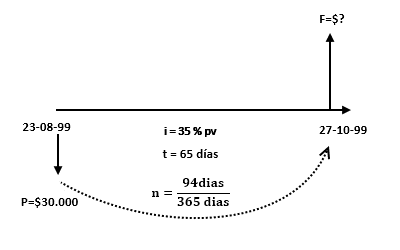
\includegraphics[height=5cm]{1_2}
\end{center}

b. Declaración de variables

%\begin{align*}
F=\$? \\ P=\$30.000 \\ i=35\% pdv \\ t=65 días\\ $n=\frac{65}{365}$ pdv
%\end{align*}

c. Declaración de fórmulas

\begin{align*}
F=P(1+in) \hspace{35 pt} \textit{Valor futuro}
\end{align*}

d. Desarrollo matemático

\begin{align*}
F=\$30.000(1 + 0,35\frac{65}{365})= \$31.869,86 \hspace{35 pt} \textit{Ecuación de valor}
\end{align*} \hspace{35 pt} 

e. Respuesta:
\\
Luego el valor final (F) es de \$31.869,86

\section{Capital inicial (P, i, n, F)}
Si despejamos P de la fórmula del monto se tiene una fórmula equivalente que nos permite calcular el valor inicial o valor presente:

\begin{align*}
	P=\frac{F}{1+in} \hspace{35 pt} \textit{Valor presente}
\end{align*}

\textbf{Ejemplo 2}
\\
¿Cuánto dinero debo depositar hoy 25 de abril en una cuenta que paga el 23\% período año vencido para que el 28 de julio pueda retirar \$60.000? Utilice año de 365 días.
\\\\
\textbf{Solución:}
\\
\textbf{a.}	Diagrama de flujo
\begin{center}
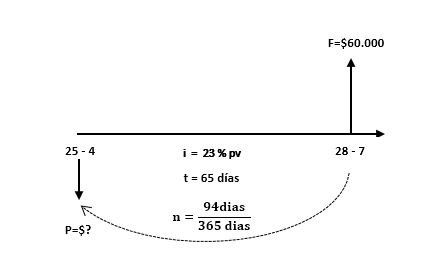
\includegraphics[height=5.1cm]{1_3}
\end{center}

\textbf{b.} Declaración de variables: \\
%\begin{align*}
P=\$?\\
F=\$60.000\\ 
$n=\frac{(94)}{(365}$pdv \\
i=23\% pdv
%\end{align*}

\textbf{c.} Declaración de formulas
\begin{align*}
P=\frac{F}{1+in} \hspace{35 pt} \textit{Valor presente de un flujo futuro (F)}
\end{align*}

\textbf{d.} Desarrollo matemático
\begin{align*}
P=\frac{\$60.000}{1+0,23  \frac{94}{365}} \hspace{35 pt} \textit{Ecuación de valor}
\end{align*}

\textbf{e.} Respuesta
El dinero que se debe depositar (P) es de \$56.644,77, \\
Justifiación: el valor Presente (p) es menor, en  valor absoluto, que el valor F de \$60.000, sin embargo estas dos sumas son equivalentes en el tiempo. 
\\\\
\textbf{Ejemplo 3}
\\
¿A qué tasa perió dica vencida, \$30.000 se convertirán en \$35.000 en 6 meses?
\\\\
\textbf{Solución:}
\\
\textbf{a.} Diagrama de flujo
\begin{center}
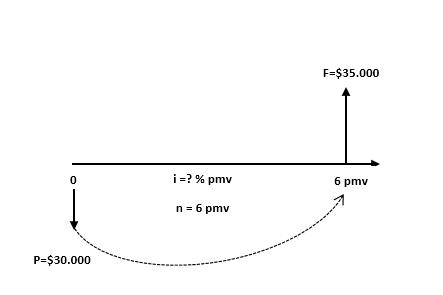
\includegraphics[height=5.1cm]{1_4}
\end{center}

\textbf{b.} Declaración de variables: \\

F=\$35.000\\
P=\$30.000 \\
i=\%? pmv\\
n=6 pmv\\


\textbf{c.} Declaración de formulas
\begin{align*}
F=P(1+in) \hspace{35 pt} \textit{Valor futuro }
\end{align*}

\textbf{d.} Desarrollo matemático
\\
despejando i:
\begin{align*}
i=\frac{F}{nP}-\frac{1}{n}=\frac{\$35.000}{(6 x \$30.000)}-\frac{1}{6}=0,3333 \Leftrightarrow 33,33\% pmv \  \hspace{35 pt} \textit{Ecuación de valor}
\end{align*}

\textbf{e.} Respuesta \\
Los \$30.000 se convertirán en \$35.000 a los 6 meses con una tasa periódica vencida de 33,33\% pmv. 

\section{Interés anticipado (I$_{a}$)}
El Interés anticipado consiste en cobrar los intereses al principio del período.

\section{Tasa anticipada (d)}
La tasa anticipada es la que genera el interés anticipado y la representaremos por $"d"$, como veremos más adelante también se le denomina tasa de descuento.

\section{Descuento simple (D)}
El descuento simple consiste en cobrar intereses por anticipado calculados sobre el valor final.
\\\\
Ya vimos que la fórmula del interés simple vencido es $I= P i n$ y por similitud, la fórmula del descuento que corresponde al interés simple anticipado será:
\begin{center}
$D=Fdn$ \hspace{35 pt} \textit{Valor de descuento}
\end{center}
Donde $D$ es la cantidad descontada.

\section{Valor líquido (VL)}
Se denomina valor líquido, valor de transacción, valor presente, valor actual o monto al valor nominal menos el descuento. De acuerdo con esta definición la fórmula del valor líquido será:
\begin{center}
$VL=F(1-dn)$ \hspace{35 pt} \textit{Valor líquido dado un flujo futuro (F)}
\end{center}

\textbf{Ejemplo 4}
\\
Supongamos que el 17 de abril de 1999 una persona necesita comprar mercancías por valor de \$800.000 para surtir su almacén y además solicita a la fábrica un plazo de 3 meses para el pago de la factura. Naturalmente que la fábrica está interesada en hacer la venta y para ello le otorgará un crédito pero le exige un documento como seguridad del pago de la deuda a su vencimiento; éste puede ser una letra que quedará en poder de la fábrica y será cobrada a su vencimiento.
\\\\
Los \$800.000 constituyen el valor nominal de la letra que tendrá por vencimiento el 17 de julio del mismo año.
\\\\
Ahora supongamos que el 20 de junio a la fábrica se le presentó un gasto inesperado y que necesita dinero en efectivo para cubrir esta contingencia; la fábrica puede ir al banco ABC a ofrecerle en venta la letra, pero es obvio que el banco no le pagará \$800.000 por el documento sino que sobre el valor nominal hará un descuento, es decir que cobrará una tasa de descuento (d).
\\\\
Ahora supongamos que el banco ABC en este tipo de operaciones cobra una tasa de descuento (d) del 36\% simple anticipado.
\\\\
¿Cuál es el valor presente de la letra, esto es cual es valor que el banco paga a la fábrica? Utilice año de 360 días.
\\\\
\clearpage
\textbf{Solución:}
\\
Entonces el primer paso para calcular el descuento será hallar los días de diferencia entre esas dos fechas.
\begin{center}
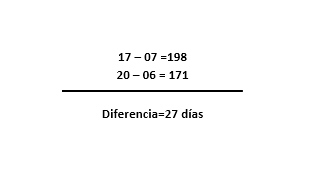
\includegraphics[height=4cm]{1_5}
\end{center}
Continuando con el problema, la gráfica de flujo de caja se presenta a continuación:
\\\\
\textbf{a. }Diagrama de flujo (del banco):
\begin{center}
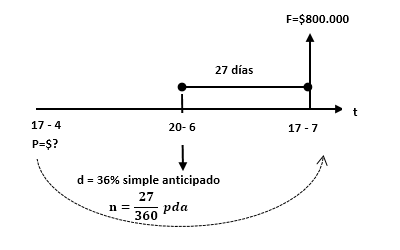
\includegraphics[height=5.1cm]{1_6}
\end{center}

\textbf{b.} Declaración de variables: \\
%\begin{align*}
P=\$?\\
F=\$800.000\\
d = 36\% simple anticipado\\
$n=\frac{27}{360}$ pda
%\end{align*}

\textbf{c.} Declaración de formulas:
\begin{align*}
VL= F(1-dn) \hspace{35 pt} \textit{Valor líquido dado un flujo futuro (F)}\\
\end{align*}

\textbf{d. }Desarrollo matemático
\begin{align*}
VL=\$800.000(1-\frac{0.36x27}{360})  = \$778.400 \hspace{35 pt} \textit{Ecuación de valor}
\end{align*}

\textbf{e.} Respuesta, el banco pagará a la fábrica la suma de \$778.400
\\\\
\textbf{Ejemplo 5}
¿Cuál debe ser el valor nominal de un documento que va a ser descontado (d) por un banco al 38\% simple anticipado entre el 17 de diciembre de 1998 y el 25 de enero de 1999 si el valor de negociación (P) es de \$637.437? Utilice año de 360 días.
\\\\
\textbf{Solución:}
calculamos los días que hay entre esas dos fechas los cuales vienen a ser 39 días.
\\
\textbf{a.} Diagrama de flujo
\begin{center}
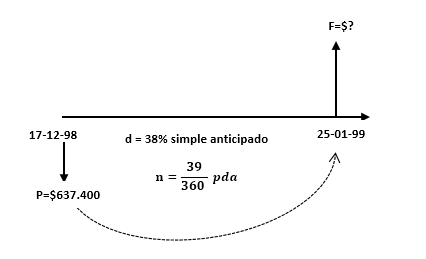
\includegraphics[height=6cm]{1_7}
\end{center}

\textbf{b. }Declaración de variables \\
%\begin{align*}
F=\$?\\
P=\$637.400\\
d=38\%\ pda\\
$n=\frac{39}{360}$pda
%\end{align*}

\textbf{c.} Declaración de formulas
\begin{align*}
P=F(1-dn) \hspace{35 pt} \textit{Valor presente de un flujo futuro (F)}\\
F=P/(1-dn) \hspace{35 pt} \textit{Valor futuro de un flujo presente (P)}\\
\end{align*}

\textbf{d.} Desarrollo matemático
\begin{align*}
F=\frac{\$637.437}{(1-0.37  \frac{39}{360})} \hspace{35 pt} \textit{Ecuación de valor}
\end{align*}

\textbf{e.} Respuesta
\\
En consecuencia el valor nominal del documento debe ser 
\$664.804,80


\section{Tasa realmente cobrada en una operación de descuento (i\%)}$(Equivalencia\  con\ la\  tasa\  de\  descuento\  [d]\  a\  la\  tasa\  de\  inter\acute{e}s\  (i\%))$


La tasa de descuento se aplica al valor final del documento, pero la tasa de interés (i\%) se aplica al valor inicial. Para calcular la tasa que realmente se cobra en una operación de descuento se aplica la fórmula del valor futuro (F).

\begin{center}
$F=P(1+in)$ \hspace{35 pt} \textit{Valor futuro}
\end{center}

\textbf{Ejemplo 6}
Una letra por valor de \$600.000 va a ser descontada por un banco 35 días antes del vencimiento al 38\%  simple anticipado. Calcular la tasa de interés periódica vencida. Utilice año de 360 días.
\\\\
\textbf{Solución}\\
\textbf{a.} Diagrama de flujo
\begin{center}
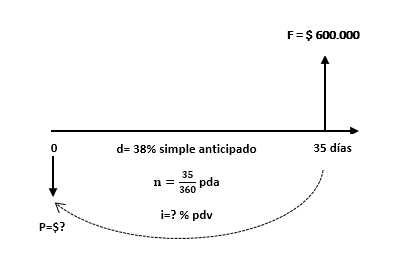
\includegraphics[height=6cm]{1_8}
\end{center}
\textbf{b.} Declaración de variables \\
%\begin{align*}
F=\$600.000\\
P=\$ ?\\
d=38\% \ da
%\end{align*}

\textbf{c.} Declaración de formulas\\
\begin{align*}
P=F(1-dn) \hspace{35 pt} \textit{Valor presente} \\
F=P(1+in)\hspace{35 pt} \textit{Valor futuro}\\
\end{align*}

\textbf{d.} Desarrollo matemático\\
\\
Igualando P de las fórmulas declaradas en el item anterior se tiene que:
P 
\begin{align*}
P=VL=\$600.000(1-0.38  \frac{35}{360})=\$577.833,33
\end{align*}
Observamos que hoy el banco invierte \$577.833,33 y a los  35 días obtiene \$600.000

\textbf{e.} Respuesta
\\
Despejando se tiene que i = 39,46\% p(35)dv
\\\\
\textbf{f.} Justificación
\\
La tasa de interés periódica y la tasa de descuento simple son equivalentes porque parten del mismo valor presente y valor futuro. Sin embargo, en términos absolutos la tasa de interés real es mayor que la tasa de descuento porque parte del valor presente (P), valor absoluto inferior del valor futuro (F).

\section{Descuentos en cadena}
Es usual que sobre una misma factura ocurran varios descuentos, tal es el caso cuando una fábrica vende mercancía a un almacén, en este caso la fábrica ofrece una serie de descuentos que son aplicables a la misma factura. Tales descuentos pueden ser:


\subsection{Descuento por volumen}
Consiste en otorgar un descuento que será progresivo conforme al valor de la factura, (en ocasiones el descuento se otorga con base en el número de unidades vendidas).

Este tipo de descuento intenta incentivar al comprador para que haga un pedido mayor con lo cual sus ganancias aumentarán al tener un mayor descuento Un ejemplo de tabla de descuento al por mayor puede ser la siguiente:

\begin{table}[H]
\fontsize{11}{9}\selectfont
\centering
\label{Descuento por volumen}
\begin{tabular}{|l|l|c|l|}
\hline
\multicolumn{2}{|c|}{Valor de la factura}                 & \multicolumn{2}{c|}{Descuento} \\ \hline
\multicolumn{2}{|c|}{Menor de \$100.000}                  & \multicolumn{2}{c|}{0\%}       \\ 
\multicolumn{2}{|c|}{Más de \$100.000 y menos de \$200.000} & \multicolumn{2}{c|}{10\%}      \\ 
\multicolumn{2}{|c|}{Más de \$200.000 y menos de \$300.000} & \multicolumn{2}{c|}{15\%}      \\
\multicolumn{2}{|c|}{Más de \$300.000 y menos de \$400.000} & \multicolumn{2}{c|}{20\%}      \\ 
\multicolumn{2}{|c|}{Más de \$400.000 y menos de \$500.000} & \multicolumn{2}{c|}{25\%}      \\
\multicolumn{2}{|c|}{Más de \$500.000}                    & \multicolumn{2}{c|}{30\%}      \\ \hline
\end{tabular}
\caption{Descuentos por volumen}
\end{table}

\subsection{Descuento por pronto pago}
Tiene por objeto incentivar al comprador a que pague lo más pronto posible, el descuento estará en relación inversa con el plazo para pagar la factura, un ejemplo de tabla puede ser:

\begin{table}[H]
\fontsize{11}{9}\selectfont
\centering
\label{Descuento por pronto pago}
\begin{tabular}{|c|l|c|l|}
\hline
\multicolumn{2}{|c|}{Plazo}      & \multicolumn{2}{c|}{Descuento} \\ \hline
\multicolumn{2}{|c|}{Al contado} & \multicolumn{2}{c|}{10\%}      \\ 
\multicolumn{2}{|c|}{30 días}    & \multicolumn{2}{c|}{6\%}       \\ 
\multicolumn{2}{|c|}{60 días}    & \multicolumn{2}{c|}{3\%}       \\ 
\multicolumn{2}{|c|}{90 días}    & \multicolumn{2}{c|}{0\%}       \\ \hline
\end{tabular}
\caption{Descuento por pronto pago}
\end{table}

\subsection{Descuento por no embalaje}
Hay almacenes que venden la mercancía empacada con el logotipo del fabricante; en ocasiones hacen el pedido y solicitan que llegue sin empacar, entonces la fábrica concede un descuento adicional igual al costo del empaque, otras veces puede ser que la mercancía llegue con un empaque más económico que el normal, o con un empaque de lujo el cual tendrá un recargo.

\subsection{Descuento por temporada}
A fin de incentivar las ventas en épocas de baja demanda las fábricas ofrecen un descuento adicional para los pedidos que sean cancelados dentro de ciertas fechas. 

\subsection{Descuento por fidelidad}
También se conoce con el nombre de descuento por antigüedad, es un pequeño porcentaje que se otorga a los clientes más leales.
\\\
Las anteriores son las principales razones para otorgar descuentos, sin embargo estos nunca se suman unos con otros sino que una vez que se aplicó el primero al saldo de la factura se le aplica el siguiente descuento y así sucesivamente hasta agotarlos todos; la respuesta final no varía si se cambia el orden de aplicar los descuentos según se puede deducir del siguiente análisis.

El descuento total será el valor nominal de la factura menos el valor de cancelación de la factura, esto es:

\begin{center}
$D=F-F(1-d_{1} )(1-d_{2} )...(1-d_{n})$

\end{center}

Esta fórmula se demuestra a través de la siguiente tabla: \\ \\

\begin{center}
\begin{table}[H]
\fontsize{11}{9}\selectfont
\centering
\begin{tabular}{@{}|c|c|c|c|@{}}
\toprule
\textbf{\begin{tabular}[c]{@{}c@{}}Valor de la Factura\\ antes del Descuento\\ {[}F{]}\\ (1)\end{tabular}} & \textbf{\begin{tabular}[c]{@{}c@{}}Tasa de \\ Descuento\\ {[}d{]}\\ (2)\end{tabular}} & \textbf{\begin{tabular}[c]{@{}c@{}}Valor del\\ Descuento\\ {[}D=Fd{]}\\ (3)\end{tabular}} & \textbf{\begin{tabular}[c]{@{}c@{}}Valor de la factura\\ después del descuento\\ {[}P = F-D = F - F  d{]}\\ (4)\end{tabular}} \\ \midrule
F                                                                                                          & $d_1$                                                                                  & $Fd_1$                                                                                      & $F-Fd_1 = F(1-d_1)$                                                                                                            \\
$F(1-d_1)$                                                                                                  & $d_2$                                                                                 & $F(1-d_1)d_2$                                                                              & \begin{tabular}[c]{@{}c@{}}$F(1-d_1) - F(1-d_1)d_2 \\= F(1-d_1)(1-d_2)$\end{tabular}
                                                                                  \\
$F(1-d_1)(1-d_2)$                                                                                          & $d_3$                                                                                  & $F(1-d_1)(1-d_2)d_3$                                                                     & \begin{tabular}[c]{@{}c@{}}$F(1-d_1)(1-d_2)-F(1-\\d_1)(1-d_2)d_3 =  F(1-d_1)(1-\\d_2)(1-d_3)$\end{tabular}                 \\
|                                                                                                          & |                                                                                     & |                                                                                          & |                                                                                                                              \\
|                                                                                                          & |                                                                                     & |                                                                                          & |                                                                                                                              \\
|                                                                                                          & |                                                                                     & |                                                                                          & |                                                                                                                              \\
|                                                                                                          & |                                                                                     & |                                                                                          & |                                                                                                                              \\

\begin{tabular}[c]{@{}c@{}}$F(1-d_1)(1-d_2)...(1-\\d_{n-1})$  \end{tabular}& $d_n$                                                                                  & \begin{tabular}[c]{@{}c@{}}$F(1-d_1)(1-d_2)...(1-\\d_{n-1})d_n$  \end{tabular}
                                                       & $F(1-d_1)(1-d_2)...(1-d_n)$                                                                                                   \\ \bottomrule
\end{tabular}
\end{table}
\end{center}


%----------------------------------------------------------------------------------------
%	INDEX
%----------------------------------------------------------------------------------------

\cleardoublepage
\phantomsection
\setlength{\columnsep}{0.75cm}
\printindex
